\documentclass[11pt]{article}
\usepackage[a4paper, margin=1in]{geometry}
\usepackage{amsmath, amssymb}
\usepackage{booktabs}
\usepackage{hyperref}
\usepackage{xcolor}
\usepackage{graphicx}
\usepackage{authblk}
\usepackage{microtype}
\usepackage[round,authoryear]{natbib}

\hypersetup{
  colorlinks = true,
  linkcolor = blue!50!black,
  citecolor = blue!50!black,
  urlcolor = blue!50!black,
}

\newcommand{\nlnr}{\texttt{no\_loops\_no\_recursion}}
\newcommand{\codecheck}[1]{\texttt{check\_#1}}

\title{Surface Tension: An Elicitation Gap, Not a Cost,\\
       Bounds Bare-Prompt Compliance with a Code-Style Constraint}
\author{Julian Quick}
\date{}

\begin{document}
\maketitle

\begin{abstract}
We ask whether small-data fine-tuning can convert a prompt-elicited code-style behavior --- writing Python without \texttt{for}/\texttt{while} loops and without recursion --- into a \emph{default} for a $31$B instruction-tuned code model (Gemma~4 31B-it) on competition-style problems (LCB-medium). We find that the bare-prompt non-compliance is, to a first approximation, an \emph{elicitation gap} rather than a cost trade-off: the constraint costs $\approx 8$ pass-rate points on average (not the $\approx 34$ a common pilot metric suggests, which is an artifact of an unreliable compliance column), and on $\approx 76\%$ of always-loop-bare problems the model produces a compliant-and-passing solution \emph{when instructed} at $n=3$ --- by rewriting the loop as a comprehension or \texttt{reduce}. We characterize the bare-prompt distribution as per-problem near-deterministic on the loop axis (the $[0.3, 0.7]$ ``discriminating zone'' is essentially empty across the base model and several fine-tunes), which is also why GRPO from base fails: every rollout group is uniform, advantage is zero. A properly-tuned LoRA SFT installs a partial loop-avoidance reflex --- generations contain \texttt{itertools} imports and ``avoid loops'' comments. The strength of the reflex depends sharply on the deploy checkpoint, and on \emph{both} a val set used for early-stopping and a clean set used for neither training nor selection the over-fit endpoint (\texttt{-final}, epoch $20$) substantially outperforms the val-NLL-minimum (\texttt{-bestval}, epoch $\approx 4$): $0.51$ vs $0.37$ on the val set, $0.26$ vs $0.09$ on the clean set. Compliance$\,\wedge\,$pass follows the same pattern. Per-problem flip rates are $75\%$ vs $67\%$ on the val set, $50\%$ vs $19\%$ on the clean set (vs $0\%$ for base). We discuss two methodological lessons: a small val set reused for early-stopping and reporting inflates apparent generalization $\approx 4\times$ at the val-min checkpoint; and val-NLL minimum is itself a poor selector for AST compliance --- the same training continued through nominal overfitting is materially better on both the set it was selected on and a clean third set.
\end{abstract}

\section{Introduction}
\label{sec:intro}

A $31$B instruction-tuned code model can comply with a stylistic AST constraint --- here, ``no \texttt{for}/\texttt{while} statements and no recursion'' --- when the rule is in the prompt, but rarely complies by default. Closing that prompt--default gap by fine-tuning is the kind of internalization task active in the capability-elicitation literature \citep{greenblatt2024passwordlocked, ryd2026sandbagging}. We probe it on Gemma~4 31B-it against LiveCodeBench-medium \citep{jain2025livecodebench}, with four contributions:

\begin{enumerate}
\itemsep0pt
\item \textbf{The gap is an elicitation gap, not a cost.} The constraint is mostly free --- $\approx 8$ pass-rate points across the LCB pilot, not the $\approx 34$ a common pilot metric reports (the metric was an artifact of treating empty AST trees as compliant). Of the $\approx 93\%$ of LCB problems where the base model loops by default, $\approx 76\%$ yield a compliant-and-passing solution when the rule is in the prompt --- usually by rewriting the loop as a list comprehension or \texttt{reduce} (\S\ref{sec:elicitation}).
\item \textbf{The bare-prompt distribution is per-problem near-deterministic.} At $T=0.7$, $8/8$ LCB problems sampled at $n \approx 14$ each fall within $0.1$ of compliance rates $0$ or $1$. On a $200$-problem expanded set, $\approx 1\%$ of problems are strictly between. This bimodality survives across the base model, an under-trained SFT, an over-trained SFT, and a KTO run (\S\ref{sec:bimodal}). It is also why GRPO from base fails: rollout groups are uniformly all-$0$ or all-$1$, advantage is zero (\S\ref{sec:grpo}).
\item \textbf{Small-data SFT installs a partial loop-avoidance \emph{reflex} whose strength depends sharply on the deploy checkpoint.} A LoRA fine-tune on $91$ (bare-prompt, compliant-completion) demonstrations covering $28$ LCB problems yields, on a $17$-problem clean set used for neither training nor selection, $\approx 0.09$ compliance at the val-NLL-minimum checkpoint (\texttt{-bestval}) but $\approx 0.26$ at the over-fit endpoint (\texttt{-final}); $0.04$ vs $0.16$ on compliance$\,\wedge\,$pass (\S\ref{sec:sft}). On the val set itself, \texttt{-bestval} reaches $0.37$ (inflated by selection on that set) and \texttt{-final} reaches $0.51$ --- so the val-NLL-minimum deploy is materially worse on \emph{both} the val set it was selected on and a clean third set. Per-problem flip rates are $67\%$ vs $75\%$ on the val set, $19\%$ vs $50\%$ on the clean set ($0\%$ for base).
\item \textbf{Methodological lesson.} The $12$ validation problems were used both to pick the deploy checkpoint (by NLL) and to report compliance. Reporting them as ``held out'' inflated the apparent generalization roughly $4\times$. Sampling $5$ further problems (the clean set) was sufficient to flip the apparent conclusion from ``SFT generalizes'' to ``small per-problem effect.'' We also report a separate trap: relying on an eval harness's ``compliant'' column that misclassified empty AST trees as compliant inflated the pilot's apparent compliance \emph{cost} by $4\times$. We recommend that any compliance figure derived from saved sources be re-checked end-to-end, and that any generalization figure not reuse problems used for checkpoint selection.
\end{enumerate}

\section{Setup}
\label{sec:setup}

\paragraph{Model and constraint.}
We use Gemma~4 31B-it (instruction-tuned, mixture-of-experts code model) in 4-bit quantization with QLoRA-style fine-tuning \citep{dettmers2024qlora, hu2022lora}. The constraint $\nlnr$ is implemented as an AST predicate: \codecheck{no\_loops} forbids \texttt{for} and \texttt{while} \emph{statements} (list/generator comprehensions, \texttt{functools.reduce}, and \texttt{itertools} builtins are permitted); \codecheck{no\_recursion} forbids self-calls within a function's own body (mutual recursion is conservatively under-flagged). Compliance is the conjunction. Constraint cost is measured against unit tests from the problem source.

\paragraph{Data and evaluation.}
We work with the LCB-medium subset from LiveCodeBench (57 problems). The SFT corpus is $146$ (bare-prompt, compliant-completion) pairs over $40$ LCB problems, generated by prompting the base model \emph{with} the constraint and keeping only the AST-compliant completions; we verified the corpus is $100\%$ compliant. We split: $91$ pairs / $28$ problems for training (\textbf{train}), $55$ pairs / $12$ problems for validation (\textbf{val}); a further $17$ LCB problems were never used for training or selection (\textbf{clean}). All evals are bare-prompt at $T=0.7$, $n=8$ unless noted, with AST compliance \emph{re-derived from saved \texttt{.py} source files}: the eval harness's CSV \texttt{compliant} column is unreliable because \codecheck{no\_loops} on an empty AST returns \texttt{True}, so \texttt{code\_extracted = 0} rows are misclassified.

\paragraph{Training.}
LoRA on stripped attention/MLP projections (Gemma 4's \texttt{Gemma4ClippableLinear} wrappers must be removed before LoRA attach: without stripping, the LoRA delta receives zero gradient because the wrapper bypasses its inner \texttt{nn.Linear}, and ``trained'' adapters are the identity --- a silent no-op that affected several prior runs in this project). We sweep $r \in \{8, 32, 128\}$ at $\alpha = 2r$, $\text{lr} = 10^{-4}$, linear-decay-to-$10\%$ schedule, $20$ epochs ($\approx 228$ optimizer steps with effective batch $8$ on $91$ training pairs); we evaluate held-out NLL every $24$ steps and save the validation-NLL-minimum checkpoint as \texttt{-bestval}. Other reported runs: $\text{lr} = 10^{-5}$ for $3$ epochs (under-trained ``v9''); $\text{lr} \in \{10^{-4}, 3\!\times\!10^{-4}\}$ for $8$/$20$ epochs (``Phase~A''); a KTO recipe \citep{ethayarajh2024kto}; and a GRPO recipe \citep{shao2024deepseekmath} from the base model.

\section{The Elicitation Gap}
\label{sec:elicitation}

We re-derive the pilot from the saved source files (Table~\ref{tab:elicitation}, Figure~\ref{fig:elicitation}). On $54$ LCB problems where both bare and constrained-prompt evals exist at $n=3$, the base model has mean pass rate $0.87$ unconstrained and $0.79$ when told ``no loops, no recursion''; on $47$ of the $49$ problems passable bare, the constraint is free ($\Delta$~pass $\approx 0$). Of $50$ always-loop-bare problems with constrained-condition data, $76\%$ ($38/50$) produce \emph{at least one compliant-and-passing} solution when the rule is in the prompt at $n=3$; the remaining $24\%$ split into ``compliant but fails'' ($6\%$, $3/50$) and ``no compliant solution found'' ($18\%$, $9/50$). The headline ``$\approx 34$-point cost'' that appears in earlier drafts of this project is an artifact of the unreliable \texttt{compliant} column (\S\ref{sec:setup}): the column treats empty AST trees as compliant, inflating both the base's apparent compliance rate and the apparent cost of the constraint.

\begin{table}[h]
\centering
\small
\begin{tabular}{lr}
\toprule
LCB problems with both bare and constrained data (base, $n=3$) & $54$ \\
Mean pass rate, bare prompt & $0.87$ \\
Mean pass rate, constrained prompt (\nlnr) & $0.79$ \\
$\Delta$ pass rate (constraint cost) & $\mathbf{-0.08}$ \\
Bare-prompt passable problems where constrained also passes & $47/49$ \\
\midrule
Bare-prompt always-loop problems (compliance $= 0$ at $n=3$) & $51/54$ \\
\quad of which constrained $\Rightarrow$ compliant-and-passing & $\mathbf{38/50}~(\mathbf{76\%})$ \\
\quad constrained $\Rightarrow$ compliant but failing tests & $3/50~(6\%)$ \\
\quad constrained $\Rightarrow$ no compliant solution found & $9/50~(18\%)$ \\
\bottomrule
\end{tabular}
\caption{Pilot, re-derived. The constraint is mostly free; bare-prompt non-compliance is largely an elicitation phenomenon. Decomposition on the $50$ always-loop-bare problems for which constrained-condition data exists. $n=3$ provides a lower bound on the recoverable fraction.}
\label{tab:elicitation}
\end{table}

\begin{figure}[h]
\centering
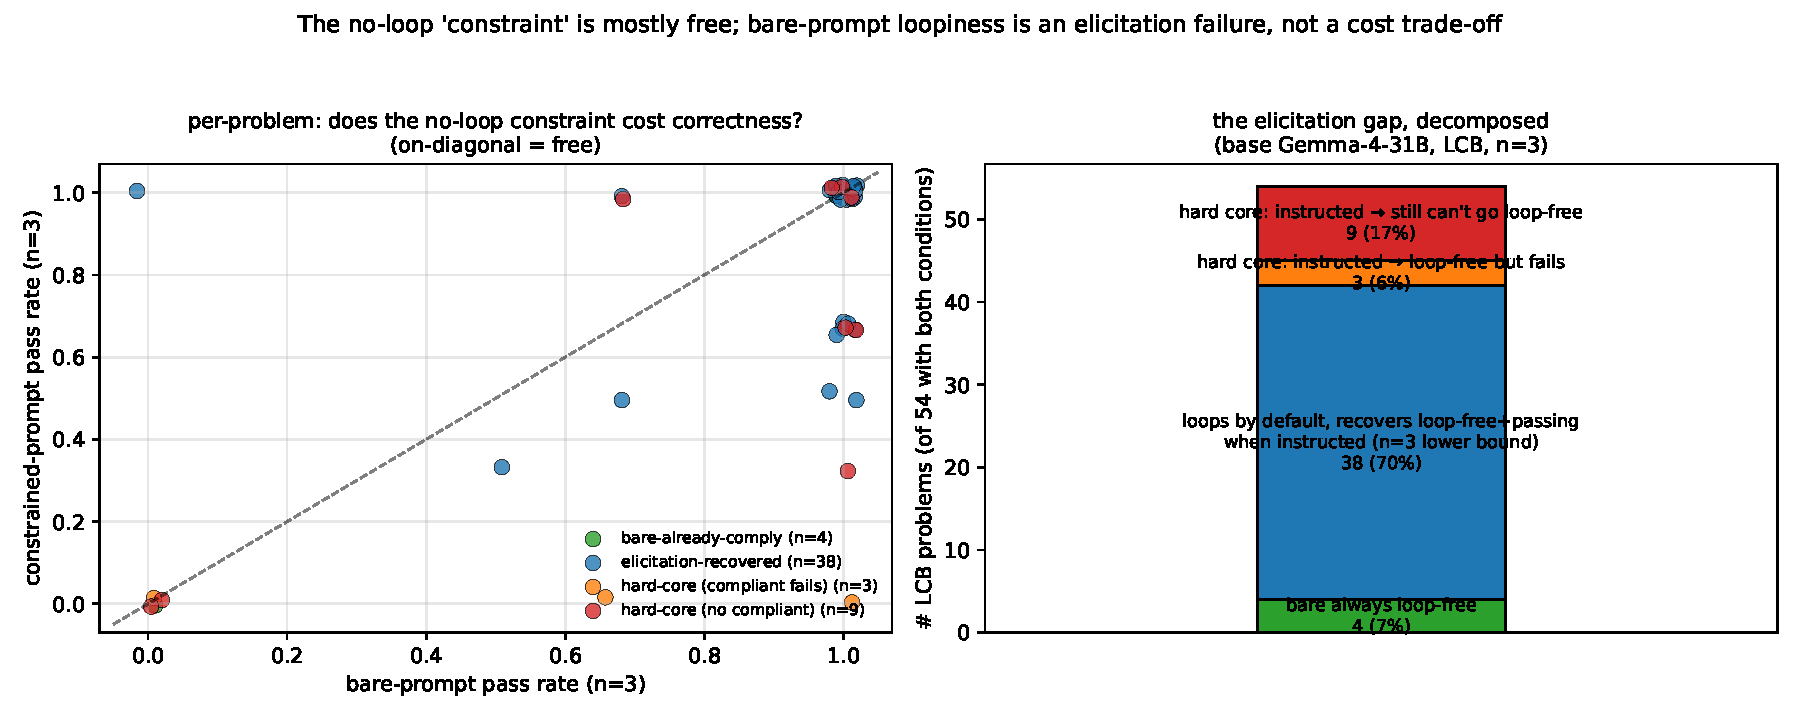
\includegraphics[width=0.95\linewidth]{figs/elicitation_gap.pdf}
\caption{\textbf{Left:} per-problem bare-prompt vs constrained-prompt pass rate; on-diagonal $=$ the constraint is free. \textbf{Right:} on $54$ LCB problems, $7\%$ already bare-compliant, $70\%$ become compliant-and-passing when instructed, $6\%$ become ``compliant but fails tests,'' and $17\%$ remain non-compliant even when told the rule (at $n=3$).}
\label{fig:elicitation}
\end{figure}

\section{Bimodal Determinism}
\label{sec:bimodal}

At $T=0.7$ the bare-prompt loop decision is per-problem near-deterministic. On $9$ LCB problems sampled at $n \in \{6, \ldots, 20\}$, $8/8$ problems with data fall within $0.1$ of compliance rate $0$ or $1$. On a $200$-problem expanded set (HumanEval + sanitized MBPP \citep{austin2021mbpp, chen2021codex}, base model), $\approx 52\%$ are always-loop, $\approx 46\%$ are always-loop-free, and only $\approx 1\%$ lie strictly in between. We re-measured the same partition under the underfit v9 SFT, the over-fit Phase~A 20-epoch checkpoint, and the KTO checkpoint: each is at most $\approx 1\%$ in the $[0.3, 0.7]$ zone. The discriminating zone is essentially empty across these models.

This is the binding precondition for verifiable-reward RL. With $G$ rollouts per prompt at $T=0.7$, a per-problem bimodal distribution means the rollout group is uniformly all-$0$ or all-$1$ on $\approx 99\%$ of prompts: GRPO's group-relative advantage is zero, no gradient. We confirmed this on a GRPO run from base: $19/19$ initial steps had advantage variance $\le 0$ (a single step had nonzero loss from an unclipped numerical edge), the mini-eval pass rate fell to $0$, and the abort fired at step $20$. We do not view this as evidence that the verifiable-reward objective is wrong; it is evidence that the precondition --- within-group reward variance --- is not satisfied by this combination of base model, constraint, and temperature.

\section{SFT: Validation vs Clean Set}
\label{sec:sft}

We trained three LoRA ranks ($r \in \{8, 32, 128\}$, $\alpha = 2r$, $\text{lr} = 10^{-4}$, linear-decay) for $20$ epochs and tracked teacher-forced NLL on the held-out $12$-problem val set every $24$ steps. The three runs are essentially indistinguishable on either curve (Figure~\ref{fig:rankcurve}): train NLL collapses toward $0$, val NLL bottoms at epoch $\approx 4$ then climbs --- the familiar U-shape. Rank is not the bottleneck. The natural deploy checkpoint is the validation-NLL minimum; we save it as \texttt{-bestval} (epoch $\approx 4$, step $48$, val NLL $\approx 0.33$ for $r=8$ and $\approx 0.35$ for $r=32$) and the over-fit endpoint as \texttt{-final}.

\begin{figure}[h]
\centering
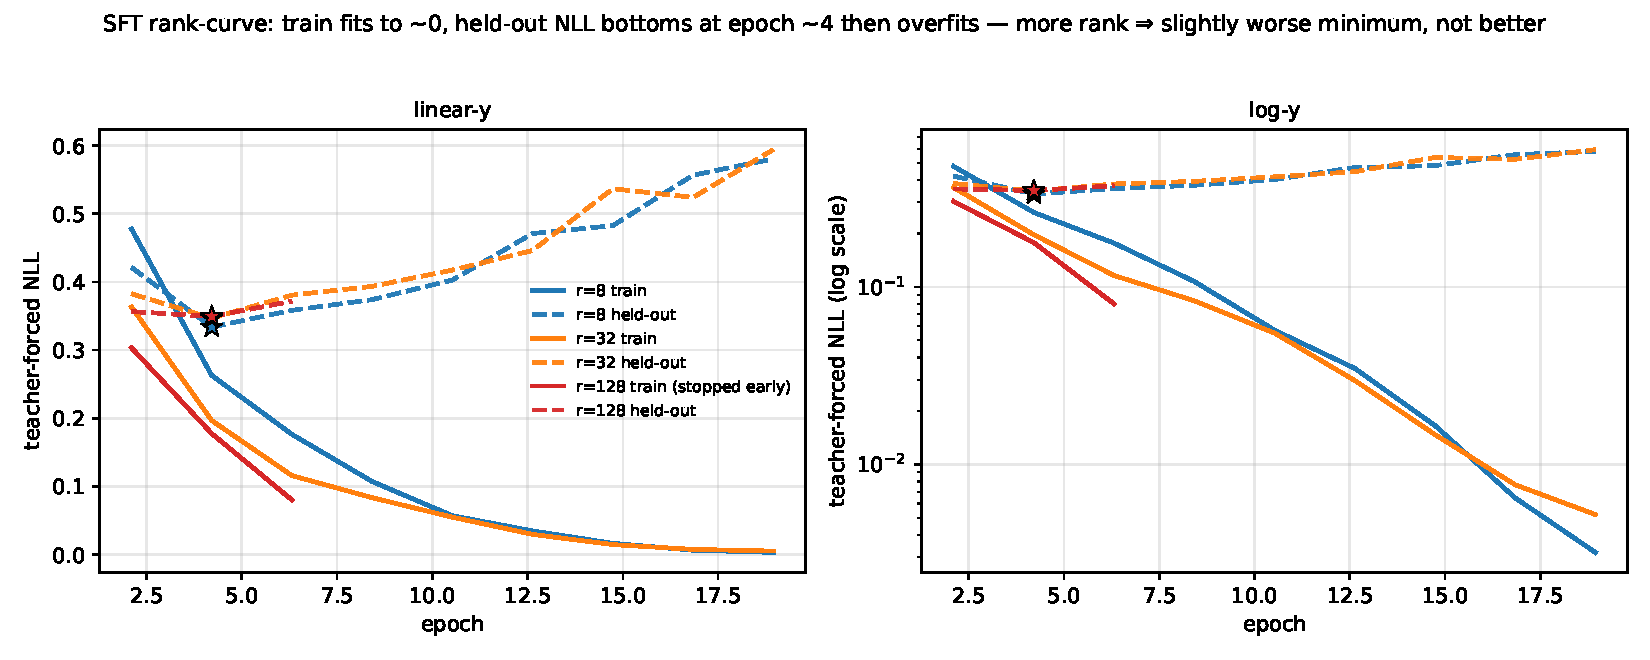
\includegraphics[width=0.95\linewidth]{figs/sft_rank_train_val.pdf}
\caption{Training-NLL (solid) and held-out-val-NLL (dashed) per epoch for $r \in \{8, 32, 128\}$. Stars mark the val-NLL minimum (the \texttt{-bestval} checkpoint). $r=128$ was halted early; $r=8$ and $r=32$ ran the full 20 epochs.}
\label{fig:rankcurve}
\end{figure}

We sample-evaluated the $r=32$ \texttt{-bestval} and \texttt{-final} checkpoints bare-prompt at $n=8$ on the $12$ val problems and the $17$ clean problems (Table~\ref{tab:sft}). The \texttt{-bestval} val-set headline is $34/93 \approx 0.37$ compliance, with $6/12$ problems strictly mixed --- a regime that does not exist for the base model or for any of v9, Phase~A, or KTO. \emph{On the clean set, the same checkpoint's compliance drops to $\approx 0.09$.} The per-problem flip rate (problems on which the base model is always-loop and the trained model produces $\ge 1$ compliant generation) is $19\%$ on the clean set, $\approx 67\%$ on the val set. Compliance$\,\wedge\,$pass is $\approx 0.04$ on the clean set --- meaning roughly half of the compliant generations \emph{fail their tests}.

\begin{table}[h]
\centering
\small
\setlength{\tabcolsep}{3.5pt}
\begin{tabular}{lcccccc}
\toprule
& base & v9 & \multicolumn{2}{c}{val set (12 prob)} & \multicolumn{2}{c}{clean set (17 prob)} \\
\cmidrule(lr){4-5} \cmidrule(lr){6-7}
& & SFT & \texttt{-bestval} & \texttt{-final} & \texttt{-bestval} & \texttt{-final} \\
\midrule
gens (usable) & $\sim n{=}3$ & $71$ & $93$ & $91$ & $70$ & $62$ \\
\textbf{compliance} & $\approx 0.05$ & $0.07$ & $\mathbf{0.37}$ & $\mathbf{0.51}$ & $0.09$ & $\mathbf{0.26}$ \\
compliance $\wedge$ pass & $\approx 0.05$ & $0.07$ & $0.34$ & $\mathbf{0.47}$ & $0.04$ & $\mathbf{0.16}$ \\
flip rate$^{*}$ & $-$ & $0/26$ & $8/12$ & $\mathbf{9/12}$ & $3/16$ & $\mathbf{6/12}$ \\
$[0.3, 0.7]$ zone & $0$ & $0$ & $2/12$ & $3/12$ & $2/17$ & $1/12$ \\
\bottomrule
\end{tabular}
\caption{Bare-prompt compliance, AST-rechecked from saved sources. $^{*}$Per-problem flip rate counts the fraction of always-loop-bare problems for which the trained model produces $\ge 1$ compliant generation. The validation set is the $12$ LCB problems used for early-stopping (so it is held out from training but not from checkpoint selection); the clean set is $17$ further LCB problems not used for either. The clean-set evals had high format-error rates ($49\%$ for \texttt{-bestval}, $54\%$ for \texttt{-final}, \texttt{no\_code\_block\_found}, concentrated on harder ``D'' problems and the \texttt{arc} problems) likely due to \texttt{max\_new\_tokens} truncation; val-set rates are $\le 6\%$ because val problems are shorter. We report compliance on usable generations. Per-problem on the clean set, \texttt{-bestval}: \texttt{abc385\_c}$=1.00$, \texttt{abc386\_c}$=0.38$, \texttt{abc379\_d}$=0.50$, \texttt{abc359\_c}$=1.00$ (already bare-compliant for base); other $13$ problems at $0.00$. Per-problem on the clean set, \texttt{-final}: $5$ new flips relative to \texttt{-bestval} (\texttt{abc362\_c}$=0.50$, \texttt{abc363\_c}$=0.12$, \texttt{abc367\_d}$=1.00$ at noisy $n{=}1$, \texttt{abc370\_c}$=0.12$, \texttt{abc379\_d}$=0.75$, \texttt{abc386\_c}$=0.86$); one regression (\texttt{abc385\_c}: $1.00\!\to\!0.00$, losing the easy closed-form flip); $5$ problems unusable due to all-gen-error truncation. Per-problem on the val set, \texttt{-final} vs \texttt{-bestval}: $4$ strong improvements (\texttt{abc356\_d}: $0.25\!\to\!0.88$; \texttt{abc377\_c}: $0.12\!\to\!0.62$; \texttt{abc384\_c}: $0.38\!\to\!0.62$; \texttt{abc367\_c}: $0.88\!\to\!1.00$); $1$ new flip (\texttt{abc372\_c}: $0\!\to\!0.14$); $1$ mild drop (\texttt{abc365\_d}: $0.57\!\to\!0.43$); $6$ stays (including $2$ saturated at $1.00$ and $3$ all-non-compliant under both).}
\label{tab:sft}
\end{table}

\paragraph{What is real qualitatively, and what is not.}
Inspecting clean-set generations: the model \emph{is} trying to avoid loops. Generations on \texttt{abc356\_c}, \texttt{abc362\_c}, \texttt{abc363\_c}, etc.\ start with \texttt{from itertools import product/permutations} or build comprehensions and contain comments like \emph{``we can't use loops, but we can use list comprehensions/max''}. The trained reflex is present and clearly distinct from base behavior. But on these harder problems the model then falls back to a \texttt{for} loop somewhere in the body; on the few problems where it does succeed (\texttt{abc385\_c}, \texttt{abc386\_c}, \texttt{abc379\_d}), the result fails tests roughly half the time. The picture is not ``SFT did nothing'' --- it installed a partial, distinguishable behavior --- but it is also not ``SFT internalized the rule.'' On the val set the model both \emph{tries} more often and \emph{succeeds} more often, because the val problems are a comprehension-friendly subset (e.g.\ cuboid-overlap is three fixed-dim $\max/\min$ comparisons; a DP recurrence on a fixed alphabet folds cleanly into \texttt{reduce}).

\paragraph{The selection caveat.}
The $12$ validation problems were used to pick \texttt{-bestval} (by NLL) and then reused to report compliance. NLL and AST compliance are correlated only weakly, so the selection pressure is mild --- but with $n=12$ problems and $\approx 4$ flips, sampling $5$ further problems (the clean set) was enough to bring the apparent generalization down by a factor of $\approx 4$. We recommend that any generalization claim for small-data fine-tuning report a clean third set whose problems were used for neither training nor checkpoint selection.

\paragraph{The val-NLL-minimum deploy is not the best checkpoint.}
We evaluated the over-fit endpoint \texttt{-final} (epoch $20$, after the val-NLL curve has fully climbed) on the same val and clean sets, expecting it to confirm the U-shape behaviorally. It did not. On the clean set, \texttt{-final} \emph{outperforms} \texttt{-bestval} by roughly $3\times$ on raw compliance ($0.26$ vs $0.09$) and $\approx 4\times$ on compliance$\,\wedge\,$pass ($0.16$ vs $0.04$). On the val set --- the set \texttt{-bestval} was selected to be best on --- \texttt{-final} also wins, $0.51$ vs $0.37$ ($+36\%$) on compliance and $0.47$ vs $0.34$ on compliance$\,\wedge\,$pass. The conditional pass rate among compliant generations is also higher under \texttt{-final} on both sets (clean: $10/16 = 62\%$ vs $3/6 = 50\%$; val: $43/46 = 93\%$ vs $32/34 = 94\%$).

The per-problem pattern is structural. On the clean set, \texttt{-final} converts $5$ previously always-loop hard problems to partial flips (\texttt{abc362\_c}, \texttt{abc363\_c}, \texttt{abc367\_d}, \texttt{abc370\_c}, \texttt{abc379\_d}) --- the comprehension-unfriendly problems \texttt{-bestval} could not crack --- and reinforces the partial flips it already had (\texttt{abc386\_c}: $0.38\!\to\!0.86$). It loses the one easy full flip \texttt{-bestval} had (\texttt{abc385\_c}: $1.00\!\to\!0.00$). On the val set, the same pattern: \texttt{-final} strongly reinforces partial flips (\texttt{abc356\_d}: $0.25\!\to\!0.88$; \texttt{abc377\_c}: $0.12\!\to\!0.62$; \texttt{abc384\_c}: $0.38\!\to\!0.62$), adds one new partial flip (\texttt{abc372\_c}: $0\!\to\!0.14$), and mildly drops one (\texttt{abc365\_d}: $0.57\!\to\!0.43$); the saturated $1.00$ problems and always-non-compliant $0.00$ problems stay where they are. The natural reading is that val-NLL minimum is a poor selector for AST-compliance generalization at this data scale: the over-fit endpoint has installed a more aggressive comprehension-rewrite reflex \emph{without} the loss-in-correctness one would expect from over-fitting, on both the val set used for selection and a clean set neither training nor selection saw.

\section{GRPO and a Cautionary Note on Hybrids}
\label{sec:grpo}

We ran GRPO with the verifiable reward $r = \mathbf{1}[\text{compliant} \wedge \text{tests~pass}]$ from the base model, $G=32$, $T=0.9$, $\text{lr} = 2\!\times\!10^{-6}$, KL anchor with weight $0.02$. The run aborted at step $20$ with mini-eval pass rate $0$. The cause is the bimodality of \S\ref{sec:bimodal}: $14/19$ steps had advantage variance $\le 0$ (uniform groups), the remaining steps had advantage variance $\le 0.06$ from very small mixed-group counts, and the policy gradient on those few non-uniform groups drove an off-manifold update that destroyed correctness. The natural next experiment is GRPO from \texttt{-bestval} rather than base: the val-set bimodality is partially broken there ($6/12$ mixed). But the clean-set bimodality is largely intact ($\approx 19\%$ flipped, of which only a few are in the discriminating zone), so the available signal from a truly OOD problem distribution is thin, and we have not run that experiment. We note two implementation issues in our GRPO code that any continuation should fix: a KL-reference path that silently fell back to the base policy when the stacked-adapter mode failed, and a raw-summed (rather than mean-normalized) gradient across active rollouts. Both have been corrected in our public code release.

\section{Discussion}
\label{sec:discussion}

Three takeaways.

\textbf{The prompt--default gap on this constraint at this scale is largely an elicitation phenomenon.} The constraint is mostly free (Table~\ref{tab:elicitation}); the bare-prompt non-compliance reflects a per-problem default rather than an inability. This is the structural cousin of password-locked-model elicitation \citep{greenblatt2024passwordlocked} --- the capability is reliably present under instruction, just inaccessible by default --- but on a stylistic AST constraint rather than a quality-locked benchmark.

\textbf{The per-problem default is near-deterministic and structurally predictable.} Bare-prompt compliance happens on problems whose loop-free solution is the natural one (closed-form, builtin-reduce, fixed-dimension max/min); always-loop problems are those whose natural framing is iterative. Training shifts the disposition (\texttt{itertools} imports become common, comprehensions are attempted) but does not reliably convert problems whose loop-free path is non-obvious; the bimodality survives most of our training attempts. The implication for verifiable-reward RL is straightforward: GRPO needs within-group reward variance, and most prompt groups don't have it; the SFT-warmstarted GRPO arm is plausible but not strongly motivated by our SFT result, since most clean-set problems remain bimodal under \texttt{-bestval}.

\textbf{Val-NLL minimum is a poor checkpoint selector for AST compliance at this data scale.} The same training run, evaluated at four points (val/clean $\times$ \texttt{-bestval}/\texttt{-final}), tells a consistent story: \texttt{-final} beats \texttt{-bestval} on \emph{both} problem sets. On the val set used for early-stopping, \texttt{-bestval} reaches $0.37$ and \texttt{-final} reaches $0.51$ ($+38\%$). On the clean set, \texttt{-bestval} drops to $0.09$ (selection inflation) and \texttt{-final} reaches $0.26$ ($\approx 3\times$). Compliance$\,\wedge\,$pass follows the same pattern. Val-NLL and AST compliance are evidently weakly correlated --- weakly enough that the deploy chosen by held-out NLL on a $12$-problem val set is materially worse than the same training continued through nominal overfitting, on \emph{both} the set it was selected on and a clean third set. We recommend reporting both deploy and overfit-endpoint numbers, and being skeptical of small-data fine-tunes that report only the val-min deploy.

\section{Limitations}
\label{sec:limitations}

One model (Gemma 4 31B-it), one constraint (\nlnr\ as operationalized by our AST checks, which permit comprehensions and \texttt{reduce}), one benchmark family (LCB-medium plus a HumanEval/MBPP partition for the bimodality measurement), small sample sizes ($n=8$ on $17$ clean problems; effective denominator on the clean-set bestval eval is $70$ after $49\%$ format errors). The format-error rate is itself a caveat: a re-run with larger \texttt{max\_new\_tokens} would recover the $4$ all-truncation problems and likely tighten the clean-set number, though the qualitative picture would survive. A stricter constraint that disallowed comprehensions and \texttt{reduce} would test a more interesting notion of ``loop-free,'' and might break the comprehension-rewrite trick at the heart of the elicitation gap; we have not tried it.

\section{Conclusion}
\label{sec:conclusion}

We frame bare-prompt non-compliance with a stylistic code constraint as an elicitation gap rather than a cost trade-off. The constraint is mostly free; the bare-prompt distribution is per-problem near-deterministic; the prompt closes most of the gap by triggering a syntactic rewrite the model already knows. A properly-tuned small-data SFT installs a partial reflex --- the model imports \texttt{itertools} unbidden and attempts comprehensions on held-out problems --- but on a truly out-of-distribution problem set it flips $\approx 19\%$ of always-loop problems to some compliance, with the rare compliant generations often producing wrong algorithms. We do not have evidence that further small-data SFT, KTO, or GRPO would meaningfully move the picture; we do have evidence that careful checkpoint reporting matters a lot, and that compliance figures derived from generated source files should be AST-rechecked end-to-end.

\bibliographystyle{plainnat}
\bibliography{refs}

\end{document}
